	\begin{figure}[H]
		\centering
 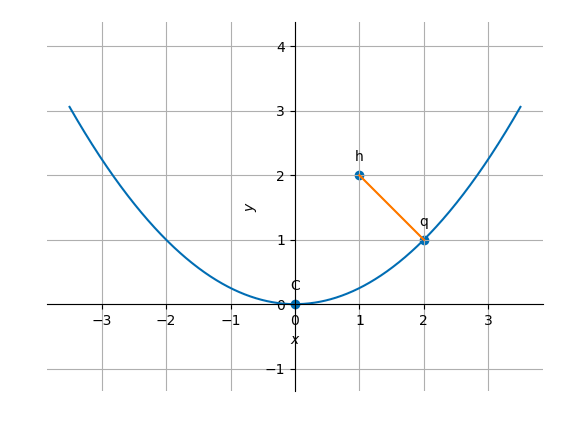
\includegraphics[width=0.75\columnwidth]{chapters/12/6/6/4/figs/conics.png}
		\caption{}
		\label{fig:12/6/6/4}
  	\end{figure}
The conic parameters are
\begin{align}
	\vec{V} = \myvec{1 & 0\\0 & 0},
	\vec{u} = \myvec{0\\-2},
	f &= 0
	%\\
\end{align}
Choosing the direction and normal vectors as
\begin{align}
	\vec{m} = \myvec{1 \\ m}, \
	\vec{n} = \myvec{-m \\ 1}, 
\end{align}
and substituting these values in
	\eqref{eq:point_of_tangency-m},
% \eqref{eq:normal_solution}, 
 we obtain
\begin{align}
m = 1
\end{align}
as the only real solution.  Thus, 
\begin{align}
%\vec{n} = \myvec{1 \\ 1},
	\vec{m} = \myvec{1 \\ 1}, 
%    \mu = -1
\end{align}
and 
	the equation of the normal is then obtained as
\begin{align}
	\vec{m}^{\top}\brak{\vec{x}-\vec{h}} &= 0
	\\
	\implies
\myvec{
1 & 1
}
		\vec{x}
	&=
\myvec{
1 & 1
}
	\myvec{1 \\2 }
	\\
	&= 3
\end{align}
		See \figref{fig:12/6/6/4}.
